\chapter {Analyzer}

Analyzer is used as a manner of facade pattern. It's role is to wrap objects and methods that compose the component and provide simple interface for a user of the analyzer. The main functionality is a processing --- analyzing --- of a single HLASM source file. Output of the analysis is data for LSP server.

\section{Overview}

\begin{figure}
	\centering
	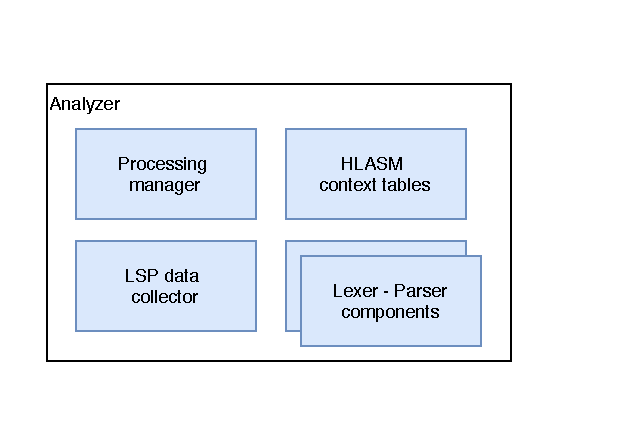
\includegraphics[width=\textwidth / 2]{img/analyzer_arch}
	\caption{The composition of Analyzer component}
	\label{fig06:analyzer}
\end{figure}

Analyzer is composed of several sub-components all required to properly process the file (see \cref{fig06:analyzer}). 
\begin{itemize}
	\item \emph{LSP data collector} collects and retieves all LSP information created while processing of the file.
	\item \emph{HLASM context tables} holds information about the context of processed HLASM source code.
	\item Analyzer facades several \emph{Lexer - Parses sub-components} to simplify the interface and ease the use of this component.
	\item \emph{Processing manager} contains the main loop where file is processed.
\end{itemize}


In order to parse a HLASM file, analyzer is constructed with contents of the file (its name and content as a string) and object that is responsible for parsing external files --- \emph{Parse library provider}. The provider is responsible for resolving source file dependencies. The dependencies are only discovered during the analysis, so it is not possible to provide the files beforehand.

In construction, analyzer creates all the mentioned subcomponents. Then, created HLASM contex tables and parser is passed to Processing manager.

When Parse library provider is called within analyzer, the second analyzer is constructed. This analyzer is ready to parse the file dependency. This \emph{inner} analysis differs from the \emph{topmost} one. The inner analyzer is passed HLASM context tables to retain the contextual consistency. Also, the inner analyzer is constructed with additional information about the library it is requested to analyze --- \emph{Library data}. The data is important for the correct functionality of the processing manager. (This recursive creation of the analyzers is bounded to the depth of 2, see ??).

To sum up, after analyzer is constructed, it analyses the source file. In result, it updated HLASM context tables and provides a list of diagnostics linked to the file, highlighting, list of symbol definitions, etc.

\section{LSP data collector}




